\documentclass{article}

\input{preamble.tex}

\title{Ejemplo de uso de \bftt{foreach} y \bftt{pic}}
\author{MSc. Fausto M. Lagos S. \\ @piratax007}
\date{\today}

\begin{document}
	\maketitle
	\thispagestyle{fancy}
	
\begin{tikzPlusCode}[Engranajes]
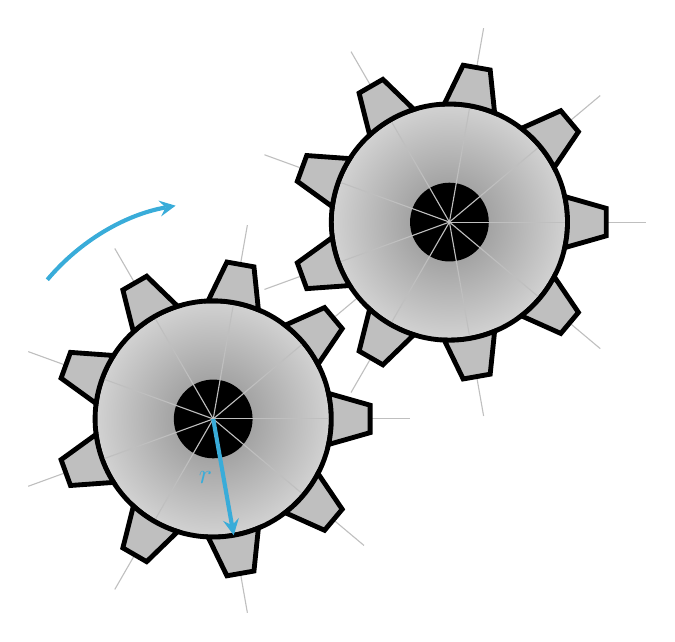
\begin{tikzpicture}[
  pieza/.pic = {\draw[fill = gray!50, line width = 1.75] (-12.5:1.5) arc[start angle = -12.5, %
    end angle = 12.5, radius = 1.5] -- (5:2) -- (-5:2) -- cycle;},
  engranaje/.pic = {
  \draw[inner color = gray!90, outer color = gray!35, line width = 1.75] (0, 0) circle[radius = 1.5];
  \fill[line width = 2] (0, 0) circle[radius = .5];
  \foreach \t in {0, 40, ..., 320}{
    \draw[gray!50] (0, 0) -- (\t:2.5); % auxiliar guides
    \pic[rotate = \t]{pieza};
  }
  }
]
\pic{engranaje};
\pic[xshift = 3cm, yshift = 2.5cm]{engranaje};
\draw[-stealth, line width = 1.5, cyan!75!gray] (0, 0) --  node[auto, left] {$r$} (-80:1.5);
\draw[-stealth, line width = 1.5, cyan!75!gray] (140:2.75) arc[start angle = 140, end angle = 100, %
 radius = 2.75];
\end{tikzpicture}
\end{tikzPlusCode}
\end{document}